% Requires graphicx; paths are relative to 11_paper/main.
% Prepared insertions; not yet included in the manuscript.
\begin{figure*}[t]
  \centering
  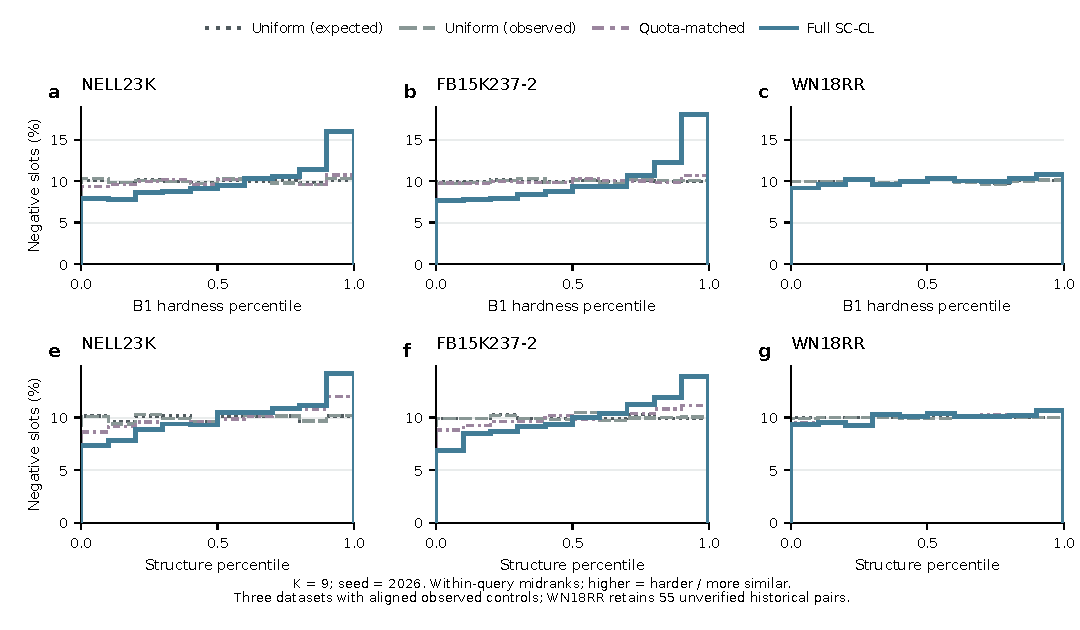
\includegraphics[width=\textwidth]{figures/sampling_diagnostics_seed2026/fig01_selection_distributions.pdf}
  \caption{Actual negative-selection distributions in four datasets.
  Within each eligible training question, legal relations are ranked by frozen
  B1 difficulty (top) and relation-profile similarity (bottom), using midranks
  for ties. Each question contributes equal mass; each actual bank contains
  nine distinct negatives (seed 2026). Expected Uniform averages all legal
  candidates analytically. CoDEx-M has no observed Uniform or quota control.
  WN18RR retains the historical pool, including 55 unverified entity pairs.
  These are generation-time diagnostics, not final-model prediction scores.}
  \label{fig:sampling-selection-signals}
\end{figure*}

\begin{figure*}[t]
  \centering
  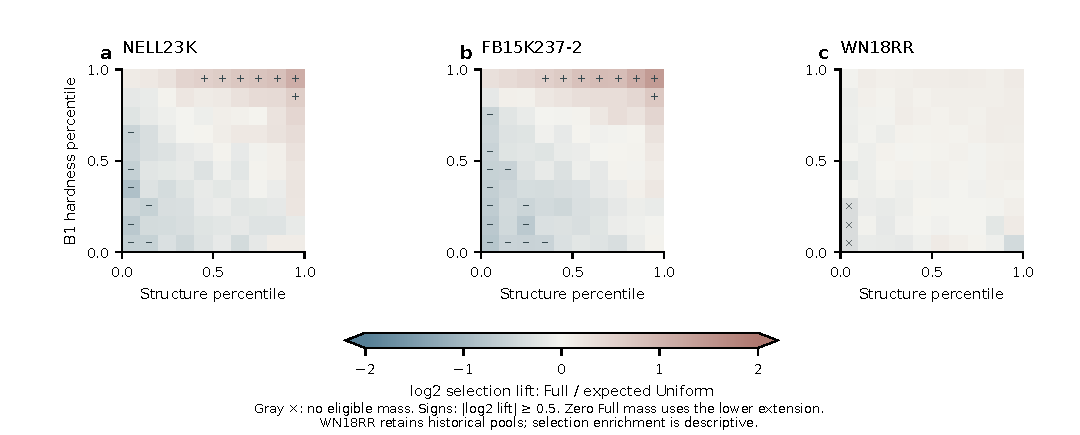
\includegraphics[width=\textwidth]{figures/sampling_diagnostics_seed2026/fig02_joint_selection_lift.pdf}
  \caption{Joint selection enrichment over the same eligible pools.
  Color shows $\log_2(P_{\mathrm{Full}}/P_{\mathrm{Uniform,expected}})$ in fixed
  structure-percentile and B1-hardness-percentile bins. Zero denotes equal
  mass; $+1$ denotes twofold enrichment. All panels share color limits
  $[-2,2]$, with extensions for values beyond the limits. Signs mark cells
  with absolute log2 lift at least 0.5. Gray crosses have no eligible mass;
  zero Full mass uses the lower extension without pseudocounts.
  Enrichment describes the sampler and does not establish causal interaction
  or downstream improvement. WN18RR is conditional on its historical pool.}
  \label{fig:sampling-joint-lift}
\end{figure*}

\begin{figure*}[t]
  \centering
  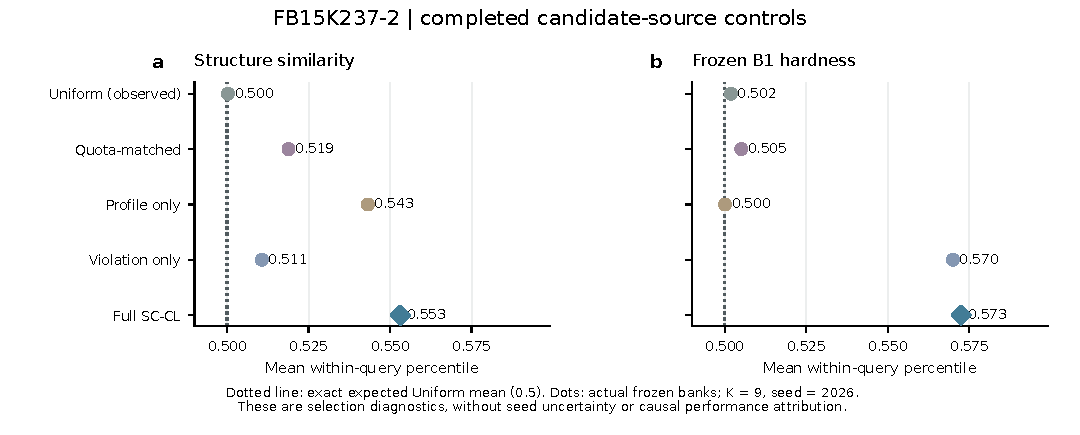
\includegraphics[width=\textwidth]{figures/sampling_diagnostics_seed2026/fig04_fb_component_fingerprints.pdf}
  \caption{Completed FB15K237-2 candidate-source controls.
  Points show actual-bank mean within-question percentiles of relation-profile
  similarity and frozen B1 difficulty. The expected Uniform mean is exactly
  0.5 on both axes. Profile-only and Violation-only alter the respective
  selection attributes, while Full shifts both. Points represent one frozen
  bank realization, without cross-seed uncertainty; selection shifts do not
  by themselves demonstrate a performance mechanism.}
  \label{fig:sampling-component-signals}
\end{figure*}

% Appendix: include fig03_relation_marginals.pdf and diagnostics_DATASET.pdf.
% All figures have editable SVG counterparts and PNG previews in this folder.
